\documentclass[12pt]{article}
\usepackage[left=1cm, right=1cm, top=2cm,bottom=1.5cm]{geometry} 

\usepackage[parfill]{parskip}
\usepackage[utf8]{inputenc}
\usepackage[T2A]{fontenc}
\usepackage[russian]{babel}
\usepackage{enumitem}
\usepackage[normalem]{ulem}
\usepackage{amsfonts, amsmath, amsthm, amssymb, mathtools,xcolor}
\usepackage{blkarray}

\usepackage{tabularx}
\usepackage{hhline}

\usepackage{accents}
\usepackage{fancyhdr}
\pagestyle{fancy}
\renewcommand{\headrulewidth}{1.5pt}
\renewcommand{\footrulewidth}{1pt}

\usepackage{graphicx}
\usepackage[figurename=Рис.]{caption}
\usepackage{subcaption}
\usepackage{float}

%%Наименование папки откуда забирать изображения
\graphicspath{ {./images/} }

%%Изменение формата для ввода доказательства
\renewcommand{\proofname}{$\square$  \nopunct}
\renewcommand\qedsymbol{$\blacksquare$}

%%Изменение отступа на таблицах
\addto\captionsrussian{%
	\renewcommand{\proofname}{$\square$ \nopunct}%
}
%% Римские цифры
\newcommand{\RN}[1]{%
	\textup{\uppercase\expandafter{\romannumeral#1}}%
}

%% Для удобства записи
\newcommand{\MR}{\mathbb{R}}
\newcommand{\MC}{\mathbb{C}}
\newcommand{\MQ}{\mathbb{Q}}
\newcommand{\MN}{\mathbb{N}}
\newcommand{\MZ}{\mathbb{Z}}
\newcommand{\MTB}{\mathbb{T}}
\newcommand{\MTI}{\mathbb{I}}
\newcommand{\MI}{\mathrm{I}}
\newcommand{\MCI}{\mathcal{I}}
\newcommand{\MJ}{\mathrm{J}}
\newcommand{\MH}{\mathrm{H}}
\newcommand{\MT}{\mathrm{T}}
\newcommand{\MU}{\mathcal{U}}
\newcommand{\MV}{\mathcal{V}}
\newcommand{\MB}{\mathcal{B}}
\newcommand{\MF}{\mathcal{F}}
\newcommand{\MW}{\mathcal{W}}
\newcommand{\ML}{\mathcal{L}}
\newcommand{\MP}{\mathcal{P}}
\newcommand{\VN}{\varnothing}
\newcommand{\VE}{\varepsilon}

\theoremstyle{definition}
\newtheorem{defn}{Опр:}
\newtheorem{rem}{Rm:}
\newtheorem{prop}{Утв.}
\newtheorem{exrc}{Упр.}
\newtheorem{lemma}{Лемма}
\newtheorem{theorem}{Теорема}
\newtheorem{corollary}{Следствие}

\newenvironment{cusdefn}[1]
{\renewcommand\thedefn{#1}\defn}
{\enddefn}

\DeclareRobustCommand{\divby}{%
	\mathrel{\text{\vbox{\baselineskip.65ex\lineskiplimit0pt\hbox{.}\hbox{.}\hbox{.}}}}%
}
%Короткий минус
\DeclareMathSymbol{\SMN}{\mathbin}{AMSa}{"39}
%Длинная шапка
\newcommand{\overbar}[1]{\mkern 1.5mu\overline{\mkern-1.5mu#1\mkern-1.5mu}\mkern 1.5mu}
%Функция знака
\DeclareMathOperator{\sgn}{sgn}

%Функция ранга
\DeclareMathOperator{\rk}{\text{rk}}

%Обозначение константы
\DeclareMathOperator{\const}{\text{const}}

\DeclareMathOperator{\codim}{\text{codim}}

\DeclareMathOperator*{\dsum}{\displaystyle\sum}
\newcommand{\ddsum}[2]{\displaystyle\sum\limits_{#1}^{#2}}

%Интеграл в большом формате
\DeclareMathOperator{\dint}{\displaystyle\int}
\newcommand{\ddint}[2]{\displaystyle\int\limits_{#1}^{#2}}
\newcommand{\ssum}[1]{\displaystyle \sum\limits_{n=1}^{\infty}{#1}_n}

\newcommand{\smallerrel}[1]{\mathrel{\mathpalette\smallerrelaux{#1}}}
\newcommand{\smallerrelaux}[2]{\raisebox{.1ex}{\scalebox{.75}{$#1#2$}}}

\newcommand{\smallin}{\smallerrel{\in}}
\newcommand{\smallnotin}{\smallerrel{\notin}}

\newcommand*{\medcap}{\mathbin{\scalebox{1.25}{\ensuremath{\cap}}}}%
\newcommand*{\medcup}{\mathbin{\scalebox{1.25}{\ensuremath{\cup}}}}%

\makeatletter
\newcommand{\vast}{\bBigg@{3.5}}
\newcommand{\Vast}{\bBigg@{5}}
\makeatother

%Промежуточное значение для sup\inf, поскольку они имеют разную высоту
\newcommand{\newsup}{\mathop{\smash{\mathrm{sup}}}}
\newcommand{\newinf}{\mathop{\mathrm{inf}\vphantom{\mathrm{sup}}}}

%Скалярное произведение
\newcommand{\inner}[2]{\left\langle #1, #2 \right\rangle }
\newcommand{\linsp}[1]{\left\langle #1 \right\rangle }
\newcommand{\linmer}[2]{\left\langle #1 \vert #2\right\rangle }

%Подпись символов снизу
\newcommand{\ubar}[1]{\underaccent{\bar}{#1}}

%% Шапка для букв сверху
\newcommand{\wte}[1]{\widetilde{#1}}
\newcommand{\wht}[1]{\widehat{#1}}

%%Трансформация Фурье
\newcommand{\fourt}[1]{\mathcal{F}\left(#1\right)}
\newcommand{\ifourt}[1]{\mathcal{F}^{-1}\left(#1\right)}

%%Символ вектора
\newcommand{\vecm}[1]{\overrightarrow{#1\,}}

%%Пространстов матриц
\newcommand{\mat}[2]{\operatorname{Mat}_{#1, #2}}


%%Взятие в скобки, модули и норму
\newcommand{\parfit}[1]{\left( #1 \right)}
\newcommand{\modfit}[1]{\left| #1 \right|}
\newcommand{\sqparfit}[1]{\left\{ #1 \right\}}
\newcommand{\normfit}[1]{\left\| #1 \right\|}

%%Функция для обозначения равномерной сходимости по множеству
\newcommand{\uconv}[1]{\overset{#1}{\rightrightarrows}}
\newcommand{\uconvm}[2]{\overset{#1}{\underset{#2}{\rightrightarrows}}}


%%Функция для обозначения нижнего и верхнего интегралов
\def\upint{\mathchoice%
	{\mkern13mu\overline{\vphantom{\intop}\mkern7mu}\mkern-20mu}%
	{\mkern7mu\overline{\vphantom{\intop}\mkern7mu}\mkern-14mu}%
	{\mkern7mu\overline{\vphantom{\intop}\mkern7mu}\mkern-14mu}%
	{\mkern7mu\overline{\vphantom{\intop}\mkern7mu}\mkern-14mu}%
	\int}
\def\lowint{\mkern3mu\underline{\vphantom{\intop}\mkern7mu}\mkern-10mu\int}

%%След матрицы
\DeclareMathOperator*{\tr}{tr}

\makeatletter
\renewcommand*\env@matrix[1][*\c@MaxMatrixCols c]{%
	\hskip -\arraycolsep
	\let\@ifnextchar\new@ifnextchar
	\array{#1}}
\makeatother

\begin{document}
\lhead{Алгебра-\RN{1}}
\chead{Тимашев Д.А.}
\rhead{Лекция - 2}

\section*{Векторные пространства}
\begin{defn}
	\uwave{Векторным пространством} называется множество $V$, элементы которого называются \uwave{векторами}, и на котором заданы $2$ алгебраические операции: сложение векторов и умножение векторов на числа, которые удовлетворяют следующим свойствам (аксиомы векторного пространства):
	\begin{enumerate}[label=\arabic*)]
		\item \textbf{Коммутативность сложения}: $u + v = v + u , \, \forall u,v \in V$;
		\item \textbf{Ассоциативность сложения}: $(u + v) + w = u + (v + w), \, \forall u,v,w \in V$;
		\item\textbf{Нулевой вектор}: $\exists \, 0 \in V \colon \forall v \in V, \, v + 0 = v$. Иногда нулевой вектор обозначают $\vecm{0}$;
		\item \textbf{Противоположный вектор}: $\forall v \in V, \, \exists \, w \in V \colon v + w = 0$. $w$ это \uwave{противоположный вектор к} $v$;
		\item \textbf{Ассоциативность умножения}: $\lambda{\cdot}(\mu{\cdot}v) = (\lambda{\cdot}\mu){\cdot}v, \, \forall v \in V,\, \forall \lambda, \mu \in \MR$;
		\item \textbf{Дистрибутивность умножения отн. векторов}: $\lambda{\cdot}(u + v) = \lambda{\cdot}u + \lambda{\cdot}v, \, \forall \lambda \in \MR, \, \forall u,v \in V$; 
		\item \textbf{Дистрибутивность умножения отн. чисел}: $(\lambda + \mu){\cdot} v = \lambda{\cdot}v + \mu{\cdot}v, \, \forall \lambda, \mu \in \MR, \, \forall v \in V$;
		\item \textbf{Нормировка}: $1{\cdot} v = v, \, \forall v \in V$;
	\end{enumerate}
\end{defn}

\subsection*{Примеры векторных пространств}
$1)$ \uwave{\textbf{Геометрическое пространство}}: $V = \{\text{геометрические векторы в пространстве (незакрепленные)}\}$.

\begin{enumerate}[label=(\arabic*)]
	\item \textbf{Вектор}: это направленный отрезок (причем незакрепленные векторы $\Leftrightarrow$ не откладываем от какой-то фиксированной точки), два вектора считаются одинаковыми если один в другой можно перевести параллельным переносом;
	
	\item \textbf{Сложение векторов}: определяется по правилу параллелограмма - откладываем два вектора от одной точки, строим на них параллелограмм, как на боковых сторонах параллелограмма. Сумма двух векторов это вектор, ведущий из этой точки в противоположную вершину параллелограмма;
	
	\item \textbf{Умножение на скаляр}: если $\lambda > 0$, то вектор будет направлен в ту же сторону, а его длина будет равна длине исходного вектора, умноженная на $\lambda$. Если $\lambda < 0$, то вектор будет направлен в противоположную сторону, а его длина будет равна длине исходного вектора, умноженная на $|\lambda|$. Если же $\lambda = 0$, то начало и конец у вектора будет в одной точке $\Rightarrow$ это будет нулевая точка;
	\begin{figure}[H]
		\centering
		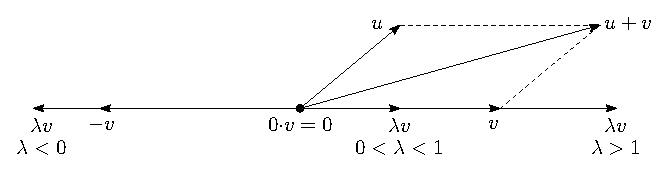
\includegraphics[width=0.7\textwidth]{AL1_1.eps}
		\caption{Геометрические векторы в пространстве: операции сложения и умножения.}
		\label{1_1}
	\end{figure}

	\item \textbf{Нулевой вектор}: это вектор начало и конец у которого совпадают;
	
	\item \textbf{Противоположный вектор}: это вектор такой же длины, но смотрящий в противоположном направлении,  в сумме с итоговым вектором, дающий ноль;
	
	\item \textbf{Аксиомы векторного пространства}: очевидно, что из геометрических соображений все аксиомы векторного пространства выполнены;
\end{enumerate}


\newpage
$2)$ \uwave{\textbf{Арифметическое векторное пространство}}, обозначение $V = \MR^n$.


\begin{enumerate}[label=(\arabic*)]
	\item \textbf{Вектор}: это упорядоченный набор (вектор или столбец) из $n$ чисел: 
	$$
		x = (x_1,\dotsc, x_n), \, x_i \in \MR, \, i = \overline{1,n}
	$$
	\item \textbf{Сложение векторов}: покомпонентное сложение чисел из двух векторов:
	$$
		\forall x = (x_1,\dotsc,x_n), \, y = (y_1,\dotsc, y_n) \in V \Rightarrow x + y = (x_1 + y_1, \dotsc, x_n + y_n)
	$$
	\item \textbf{Умножение на скаляр}: покомпонентное умножение числа $\lambda$ на числа из вектора:
	$$
		\forall \lambda \in \MR, \, \forall x = (x_1,\dotsc,x_n) \in V, \, \lambda{\cdot}x = (\lambda{\cdot}x_1, \dotsc, \lambda{\cdot}x_n)
	$$
	\item \textbf{Аксиомы векторного пространства}: аксиомы выполнены, поскольку операции над строками или столбцами производятся покомпонетно, то есть отдельно на каждой компоненте и эти свойства сводятся к отдельным операциям над числами, а над числами все эти свойства выполнены;
	
	\item \textbf{Нулевой вектор}: $\vecm{0} = (0, 0 ,\dotsc,0)$;
	
	\item \textbf{Противоположный вектор}: $x = (x_1,\dotsc,x_n) \Rightarrow (-x_1,-x_2, \dotsc, -x_n)$;
\end{enumerate}


$3)$ \uwave{\textbf{Пространство функций на множестве}} $X$, $V = \MF(X,\MR) =\{f \colon X \to \MR \}$ - функции на $X$.

\begin{enumerate}[label=(\arabic*)]
	\item \textbf{Вектор}: функция $f \colon X \to \MR$;
	
	\item \textbf{Сложение векторов}: 
	$$
		\forall f,g \in \MF(X,\MR) \Rightarrow (f+g)(x) = f(x) + g(x), \, \forall x \in \MR
	$$
	
	\item \textbf{Умножение на скаляр}: 
	$$
		\forall \lambda \in \MR, \, \forall f \in \MF(X,\MR) \Rightarrow \lambda{\cdot}f(x)
	$$
	
	\item \textbf{Аксиомы векторного пространства}: легко видеть, что все аксиомы будут выполнены;
	
	\item \textbf{Нулевой вектор}: $f \equiv 0 \Rightarrow \forall x \in \MR, \, 0(x) = 0$;
	
	\item \textbf{Противоположный вектор}: $f \in \MF(X,\MR) \Rightarrow g \in \MF(X,\MR) \colon g(x) = -f(x), \, \forall x \in \MR$;
\end{enumerate}


\subsection*{Свойства векторных пространств}
\begin{prop}(\textbf{Единственность нулевого вектора})
	Нулевой вектор единственен.
\end{prop}
\begin{proof}
	Пусть $0'$ - другой нулевой вектор, сложим их:
	$$
		0 + 0' = 0		
	$$
	Так как $0'$ - нулевой вектор. С другой стороны, $0$ - тоже нулевой вектор, поэтому:
	$$
		0 + 0' = 0' \Rightarrow  0 = 0 + 0' = 0' \Rightarrow 0 = 0'
	$$
\end{proof}

\begin{prop}(\textbf{Единственность противоположного вектора})
	$\forall v \in V, \, \exists! \, w \in V \colon v + w = 0$.
\end{prop}
\begin{proof}
	Пусть $w'$ - другой вектор, противоположный $v$, рассмотрим тройную сумму:
	$$
		w+ v + w' \colon (w + v) + w' = 0 + w' = w', \, w + (v + w') = w + 0 = w \Rightarrow
	$$
	$$
		\Rightarrow  w = w + 0 = w + (v + w') = (w + v) + w' = 0 + w' = w' \Rightarrow w = w'
	$$
\end{proof}

В силу единственности противоположного вектора, как-то канонически обозначим его.

\uline{\textbf{Обозначение для противоположного вектора}}: $w = -v$.

\begin{prop}
	$\forall  v \in V,\,  0 {\cdot} v = \vecm{0}$.
\end{prop}
\begin{proof}
	Рассмотрим это произведение и представим $0$ как сумму нулей:
	$$
		\forall v \in V, \, 0{\cdot}v = (0 + 0){\cdot}v = 0{\cdot}v + 0{\cdot}v \Rightarrow 
	$$
	$$
		\Rightarrow 0{\cdot}v + (-0{\cdot}v) = 0{\cdot}v + 0{\cdot}v + (-0{\cdot}v) \Leftrightarrow \vecm{0} = 0{\cdot}v + \vecm{0} = 0{\cdot}v \Rightarrow 0 {\cdot} v = \vecm{0}
	$$
\end{proof}

\begin{prop}
	$\forall \lambda \in \MR, \, \lambda{\cdot}\vecm{0} = \vecm{0}$.
\end{prop}
\begin{proof}
	По аналогии выше:
	$$
		\forall \lambda \in \MR, \, \lambda{\cdot}\vecm{0} = \lambda{\cdot}(\vecm{0} + \vecm{0}) = \lambda{\cdot}\vecm{0} + \lambda{\cdot}\vecm{0} \Rightarrow
	$$
	$$
		\Rightarrow  \lambda{\cdot}\vecm{0} + (-\lambda{\cdot}\vecm{0}) = \lambda{\cdot}\vecm{0} + \lambda{\cdot}\vecm{0}+ (-\lambda{\cdot}\vecm{0}) \Leftrightarrow \vecm{0} = \lambda{\cdot}\vecm{0} + \vecm{0} = \lambda{\cdot}\vecm{0} \Rightarrow \lambda{\cdot}\vecm{0} = \vecm{0}
	$$
\end{proof}

\begin{prop}
	$\forall v \in V, \,(-1){\cdot}v = - v$.
\end{prop}
\begin{proof}
	Проверим, что написанный вектор является противоположным.
	$$
		v + (-1){\cdot}v = 1{\cdot}v + (-1){\cdot}v = (1 + (-1)){\cdot} v = 0{\cdot}v = \vecm{0}
	$$
	А это и означает по определению, что $(-1){\cdot}v = -v$.
\end{proof}
\newpage

\section*{Линейная зависимость}
\begin{defn}
	\uwave{Линейная комбинация} векторов $v_1, \dotsc, v_m \in V$ с коэффициентами $\lambda_1,\dotsc, \lambda_m \in \MR$ это выражение следующего вида:
	$$
		\lambda_1 {\cdot}v_1 + \lambda_2 {\cdot} v_2 + \dotsc + \lambda_m {\cdot} v_m
	$$
	Её значение это тоже вектор из пространства $V$.
\end{defn}
\begin{defn}
	Линейная комбинация называется \uwave{тривиальной}, если $\lambda_1 = \lambda_2 = \dotsc = \lambda_m = 0$. Значение тривиальной линейной комбинации равно $\vecm{0}$. В противном случае, она называется \uwave{нетривиальной}.
\end{defn}

\begin{defn}
	Система векторов $S = \{v_1,\dotsc, v_m\}$ называется \uwave{линейно зависимой}, если существует нетривиальная линейная комбинация этих векторов, которая равна нулю:
	$$
		\exists \, i \colon \lambda_i \neq 0, \, \lambda_1 v_1 + \dotsc + \lambda_m v_m = \vecm{0}
	$$
	В противном случае, система называется \uwave{линейно независимой}
\end{defn}

\textbf{Пример}: $S = \{v\} \Rightarrow$ эта система линейно зависима $\Leftrightarrow v = \vecm{0}$. 
\begin{proof}\hfill\\
	$(\Rightarrow)$ В самом деле: $\exists \, \lambda \neq 0 \colon \lambda{\cdot}v = \vecm{0}$, умножим равенство на число обратное к $\lambda$, тогда:
	$$
		\dfrac{1}{\lambda}{\cdot}\lambda{\cdot}v = \dfrac{1}{\lambda}{\cdot}\vecm{0} = \vecm{0} \Leftrightarrow v = \vecm{0}
	$$
	$(\Leftarrow)$ Обратно: $v = \vecm{0} \Rightarrow 1{\cdot}\vecm{0} = \vecm{0}$ - нетривиальная лин. комбинация $\Rightarrow S = \left\{\vecm{0}\right\}$ - линейно зависима.
\end{proof}

\textbf{Пример}: $S = \{v_1, v_2\}$ - линейно зависима $\Leftrightarrow$ когда векторы пропорциональны, то есть $v_1 = k v_2$.
\begin{proof}\hfill\\
	$(\Rightarrow)$ Пусть $\lambda_1 v_1 + \lambda_2 v_2 = \vecm{0}$ - нетривиальная лин. комбинация, можно считать без ограничения общности, что $\lambda_1 \neq 0$, тогда:
	$$
		\lambda_1 v_1 = - \lambda_2 v_2 \Rightarrow v_1 = \left(-\dfrac{\lambda_2}{\lambda_1}\right)v_2
	$$
	$(\Leftarrow)$ Если $v_1 \sim v_2$, то без ограниения общности можно считать, что $v_1 = \mu{\cdot}v_2$, тогда:
	$$
		1{\cdot}v_1 + (-\mu){\cdot}v_2 = \vecm{0}
	$$
	Таким образом, мы получили нетривиальную линейную комбинацию, поскольку $1\neq 0 \Rightarrow$ система векторов $\{v_1,v_2\}$ - линейно зависима.
\end{proof}

\subsection*{Свойства линейной зависимости}
\begin{prop}
	Если система векторов $S$ - линейно зависима, $S \subset S' \Rightarrow S'$ - линейно зависима. 
\end{prop}
\begin{proof}
	Пусть $S = \{v_1,\dotsc, v_m\}, \, S' = \{v_1,\dotsc,v_m, v_{m+1},\dotsc, v_n\}$. Поскольку $S$ - линейно зависима, то $\exists$ нетривиальная линейная комбинация $\lambda_1 v_1 + \dotsc + \lambda_m v_m = 0 \Rightarrow$ можем добавить к этим слагаемым оставшиеся векторы из $S'$ с нулевыми коэффициентами:
	$$
		\lambda_1 v_1 + \dotsc + \lambda_m v_m + 0{\cdot}v_{m+1} + \dotsc + 0{\cdot}v_n = 0
	$$
	Это будет нетривиальной линейной комбинацией векторов из системы $S'$, потому что осталась нетривиальная комбинация из $S \Rightarrow S'$ - линейно зависима.
\end{proof}

\begin{prop}
	Если система векторов $S$ - линейно независима, $\forall S' \subset S \Rightarrow S'$ - линейно независима.	
\end{prop}
\begin{proof}
	Пусть это не так и $S'$ - линейно зависима, тогда по предыдущему утверждению $S$ - тоже была бы линейно зависимой, поскольку $S' \subset S \Rightarrow S'$ линейно независима. 
\end{proof}

\begin{defn}
	Говорят, что вектор $v \in S$ \uwave{линейно выражается} через оставшиеся векторы системы $S$, если существует линейная комбинация векторов из $S \setminus \{v\}$ равная $v$:
	$$
		\exists \, v_1 ,\dotsc, v_m \in S \setminus \{v\}, \, \lambda_1 ,\dotsc, \lambda_m \in \MR \colon v = \lambda_1 v_1 + \dotsc + \lambda_m v_m
	$$
\end{defn}
\begin{prop}
	Система векторов $S$ линейно зависима $\Leftrightarrow \exists \, v \in S \colon v$ представляется в виде линейной комбинации векторов из оставшейся системы: $S \setminus \{v\}$ (линейно выражается через оставшиеся векторы). 
\end{prop}
\begin{proof}\hfill\\
	$(\Rightarrow)$ Пусть $S = \{v_1,\dotsc, v_m\}$ - линейно зависима, тогда существует нетривиальная линейная комбинация этих векторов равная $0$:
	$$
		\exists \lambda_i \neq 0, \, \lambda_1 v_1 + \dotsc + \lambda_m v_m = 0
	$$	
	Перенесем все слагаемые, кроме $i$-го перенсти в правую часть и поделим на $\lambda_i$:
	$$
		v_i = \left(-\dfrac{\lambda_1}{\lambda_i}\right){\cdot}v_1 + \dotsc + \left(-\dfrac{\lambda_{i-1}}{\lambda_i}\right){\cdot}v_{i-1} + \left(-\dfrac{\lambda_{i+1}}{\lambda_i}\right){\cdot}v_{i + 1} + \dotsc + \left(-\dfrac{\lambda_m}{\lambda_i}\right){\cdot}v_m
	$$
	То есть, $v_i$ линейно выражается через векторы $S \setminus \{v_i\}$.
	
	$(\Leftarrow)$ Пусть $v_i = \mu_1 v_1 + \dotsc + \mu_{i-1}v_{i-1} + \mu_{i+1}v_{i+1} + \dotsc + \mu_m v_m$, перенесём все слагаемые и получим:
	$$
		\mu_1 v_1 + \dotsc + \mu_{i-1}v_{i-1} + (-1){\cdot}v_i + \mu_{i+1}v_{i+1} + \dotsc + \mu_m v_m = 0
	$$
	Следовательно, мы получили нетривиальную линейную комбинацию векторов из $S$, которая равна $0 \Rightarrow$ система $S$ - линейно зависима.
\end{proof}
\begin{prop}
	Предположим, что система векторов $S$ - линейно независима, но $S \cup \{v\}$ - линейно зависима, тогда $v$ линейно выражается через $S$, причем единственным способом.
\end{prop}
\begin{proof}
	Обозначим $S = \{v_1, \dotsc, v_m\} \Rightarrow \exists$ нетривиальная линейная комбинация:
	$$
		\lambda_1{\cdot} v_1 + \dotsc + \lambda_m{\cdot} v_m + \lambda{\cdot}v = 0
	$$
	Тогда $\lambda \neq 0$ иначе мы бы получили нетривиальную систему: $\lambda_1{\cdot} v_1 + \dotsc + \lambda_m{\cdot} v_m = 0 \Rightarrow$ система $S$ была бы линейно зависима, вопреки условию. Следовательно, аналогично предыдущему утверждению:
	$$
		v = \left(-\dfrac{\lambda_1}{\lambda}\right){\cdot}v_1 + \dotsc  + \left(-\dfrac{\lambda_m}{\lambda}\right){\cdot}v_m
	$$
	В результате, $v$ линейно выражается через векторы системы $S$. Проверим, что он выражается единственным способом. Пусть вектор $v$ представляется неоднозначно:
	$$
		v = \alpha_1 {\cdot}v_1 + \dotsc + \alpha_m v_m = \beta_1 v_1 + \dotsc + \beta_m v_m \Rightarrow (\alpha_1 - \beta_1){\cdot}v_1 + \dotsc + (\alpha_m- \beta_m){\cdot}v_m = 0
	$$
	Поскольку $S$ - линейно независима, то линейная комбинация векторов из $S$ может быть только тривиальной, следовательно:
	$$
		\alpha_1 - \beta_1 = 0, \dotsc, \alpha_m - \beta_m = 0 \Rightarrow \alpha_1 = \beta_1 , \dotsc, \alpha_m = \beta_m
	$$
	И таким образом, представление единственное.
\end{proof}
\newpage
\begin{rem}
	Заметим, что линейная зависимость векторов $v_1,\dotsc, v_k$ не означает, что любой из них выражается через остальные. Например, $V = \MR^2$ с векторами:
	$$
		v_1 = (1,0), \, v_2 = (0,1),\, v_3 = (0,2) \Rightarrow 0{\cdot}v_1 + 2{\cdot}v_2 + (-1){\cdot}v_3 = 0
	$$
	Из этой линейной комбинации выразить $v_1$ нельзя.
\end{rem}
\begin{theorem}(\textbf{Основная лемма о линейной зависимости})\\
	Пусть $S = \{v_1,\dotsc, v_n\}, \, T = \{w_1,\dotsc, w_m\}$ - две системы векторов, причем система $S$ линейно выражается через систему $T$ и в системе $S$ больше векторов, чем в $T$ ($n > m$). Тогда $S$ линейно зависима.
\end{theorem} 
\begin{rem}
	Можно теорему переформулировать так: Если система $S$ линейно выражается через систему $T$ и система $S$ линейно независима, то в ней векторов не больше, чем в $T$ ($n\leq m$).
\end{rem}
\begin{proof}
	По условию $\forall j = \overline{1,n}, \, v_j = a_{1j}{\cdot}w_1 + a_{2j}{\cdot}w_2 + \dotsc + a_{mj}{\cdot}w_m$. Найдем нетривиальную линейную комбинацию векторов из $S$, равную нулю. Для этого рассмотрим их произвольную линейную комбинацию:
	$$
		\lambda_1{\cdot} v_1 + \lambda_2{\cdot} v_2 + \dotsc+ \lambda_n{\cdot} v_n = \ddsum{j = 1}{n}\lambda_j{\cdot}\ddsum{i = 1}{m}a_{ij}w_i = \ddsum{\substack{i = 1,\dotsc,m\\j = 1,\dotsc, n}}{}a_{ij}{\cdot}\lambda_j{\cdot}w_i = \ddsum{i = 1}{m}\left(\ddsum{j = 1}{n}a_{ij}\lambda_j\right){\cdot}w_i
	$$
	Следовательно, линейную комбинацию векторов из системы $S = \{v_1,\dotsc, v_m\}$ переписали в виде линейной комбинации векторов из системы $T = \{w_1,\dotsc, w_m\}$. Рассмотрим ОСЛУ у которой матрица коэффициентов будет составлена из $\{a_{ij}\}$:
	$$
		\left\{
			\begin{array}{ccccccccc}
				a_{11}x_1 & + & a_{12}x_2 & + & \dotsc & + & a_{1n}x_n & = & 0 \\
				a_{21}x_1 & + & a_{22}x_2 & + & \dotsc & + & a_{2n}x_n & = & 0 \\
				\vdots & \vdots & \vdots & \vdots & \ddots & \vdots & \vdots & \vdots & \vdots \\ 
				a_{m1}x_1 & + & a_{m2}x_2 & + & \dotsc & + & a_{mn}x_n & = & 0 
			\end{array}
		\right.
	$$
	По условию у нас $n > m \Leftrightarrow$ уравнений меньше, чем неизвестных $\Rightarrow$ как мы уже знаем, существует ненулевое решение: $x_1 = \lambda_1 , x_2 = \lambda_2, \dotsc, x_n = \lambda_n \Rightarrow$ при подстановке в уравнения даст верные равенства:
	$$
		\ddsum{j = 1}{n}a_{ij}\lambda_j = 0, \, \forall i = \overline{1,m} \Rightarrow \ddsum{i = 1}{m}\left(\ddsum{j = 1}{n}a_{ij}\lambda_j\right){\cdot}w_i = 0 \Rightarrow 	\lambda_1{\cdot} v_1 + \lambda_2{\cdot} v_2 + \dotsc+ \lambda_n{\cdot} v_n = 0 
	$$
	Но при этом, поскольку решение мы взяли ненулевое, то $\exists \, \lambda_i \neq 0 \Rightarrow$ система $S$ - линейно зависима.
\end{proof}
\begin{rem}
	Понятия линейной комбинации, линейной зависимости, линейного выражения одних векторов через другие можно обобщить на бесконечные системы векторов.
	
	\uwave{Линейная комбинация}: $\ddsum{i \in \MI}{}\lambda_i{\cdot}v_i$, система векторов $S = \{v_i \mid i \in \MI\}$ имеет смысл если $\lambda_i = 0, \, \forall i \in \MI$, кроме конечного количества $\Rightarrow$ ненулевых лишь конечное число слагаемых. 
	
	В этом случае свойства линейной зависимости переносятся без изменений на бесконечные системы векторов, поскольку всё сводится к конечным подсистемам.
\end{rem}

\end{document}